\section{Технологический раздел}

\subsection{Выбор СУБД}

При выборе СУБД для решения поставленной задачи можно выделить следующие критерии:

\begin{enumerate}[left=0.49cm, label*=---]
	\item открытый исходный код;
	\item опыт работы;
        \item возможность создания триггеров.
\end{enumerate}

Результаты сравнения наиболее популярных СУБД по указанным критериям приведены в таблице \ref{tab:dsms}.

\begin{table}[hbtp]
	\begin{center}
			\caption{\label{tab:dsms}Сравнение СУБД}
		\begin{tabular}{|l|l|l|l|l|l|l|l|}
			\hline {СУБД} & {Критерий 1} & {Критерий 2} & {Критерий 3}\\ \hline
			 PostgreSQL~\cite{postgres} & + & + & + \\ \hline
            MySQL~\cite{mysql} & + & - & + \\ \hline
            Oracle~\cite{oracle} & - & - & + \\ \hline
		\end{tabular}
	\end{center}
\end{table}

По результатам сравнения в данной работе будет использоваться СУБД PostgreSQL.



\subsection{Средства реализации}
Для реализации приложения использовались следующие технологии.

\begin{enumerate}[left=0.49cm, label=\arabic*.]
	\item Язык программирования --- Golang~\cite{golang}.
        \item Система управления базами данных --- PostgeSQL.
	\item Драйвер для работы с СУБД PostgreSQL --- pgx~\cite{pgx}.
        \item Фреймворк для реализации API --- gin~\cite{gin}.
        \item ПО для развертывания приложения --- Docker~\cite{docker}.
        \item Фреймворк для документации REST API --- Swagger~\cite{swagger}.
\end{enumerate}


\newpage
\subsection{Детали реализации}

\subsubsection{Таблицы базы данных}

В листингах \ref{t1}---\ref{t4} представлен код создания таблиц, спроектированных в конструкторской части.

\lstinputlisting[label=t1, caption=Скрипт создания таблиц (часть 1)]{code/t1.sql}
\clearpage

\lstinputlisting[label=t2, caption=Скрипт создания таблиц (часть 2)]{code/t2.sql}
\clearpage

\lstinputlisting[label=t3, caption=Скрипт создания таблиц (часть 3)]{code/t3.sql}
\clearpage

\lstinputlisting[label=t4, caption=Скрипт создания таблиц (часть 4)]{code/t4.sql}

\subsubsection{Роли базы данных}

В листинге \ref{r1} представлен код создания ролей и выделения им прав, соответствующих разработанной в конструкторской части ролевой модели.
\clearpage

\lstinputlisting[label=r1, caption=Скрипт создания ролевой модели базы данных]{code/r1.sql}

\subsubsection{Триггер базы данных}

В листингах \ref{tr1}, \ref{tr2} представлен код триггера и соответствующей функции, разработанной в конструкторской части.

\lstinputlisting[label=tr1, caption=Триггер базы данных (часть 1)]{code/tr1.sql}
\clearpage

\lstinputlisting[label=tr2, caption=Триггер базы данных (часть 2)]{code/tr2.sql}


\subsection{Тестирование}

Тестирование компонента бизнес---логики выполнялось с использованием пакета Testing~\cite{testing}. Для тестирования были написаны модульные тесты с использованием библиотеки Gomock~\cite{gomock}, которая позволяет использовать заглушки, с помощью которых были реализованы тесты.

Так же были написаны интеграционные тесты для связи компонента бизнес---логики и компонента доступа к данным с использованием пакета Testing.


\subsection{Интерфейс приложения}

Приложение является web---сервером, взаимодействие с которым может быть реализовано через интерфейс REST API. Описание REST API приложения представлено в таблице \ref{tbl:rest-api}.

\newpage
\begin{landscape}
	\begin{longtable}{|p{0.45\textwidth}|p{0.11\textwidth}|p{0.865\textwidth}|}
		\caption[Описание REST API реализуемого приложения]{Описание REST API реализуемого приложения}
		\label{tbl:rest-api}\\
		\hline
		Путь & HTTP-метод & Описание \\
		\endfirsthead
		
		\multicolumn{3}{l}
		{{\tablename\ \thetable{} -- продолжение}} \\\hline 
		Путь & Метод & Описание \\
		\endhead
		
		\multicolumn{3}{|r|}{{Продолжение на следующей странице}} \\ \hline
		\endfoot
		
		\hline \multicolumn{3}{|r|}{{Конец таблицы}} \\ \hline
		\endlastfoot
		\hline
		/api/v1/login         		& POST 		& Вход в систему \\\hline
		/api/v1/logout            	& POST 		& Выход из системы \\\hline
		
		/api/v1/leaders    		& GET 		& Получение всех руководителей  \\\hline
		/api/v1/leader/\{expedition\_id\}    		& GET 		& Получение руководителей заданной экспедиции  \\\hline
            /api/v1/leader    		& POST 		& Добавление  руководителя  \\\hline
            /api/v1/leader\_expedition    		& POST 		& Добавление  связи руководителя и экспедиции  \\\hline
            /api/v1/leader/\{id\}    		& DELETE 		& Удаление  руководителя по идентификатору  \\\hline
		
		/api/v1/members    		& GET 		& Получение всех участников  \\\hline
		/api/v1/member/\{expedition\_id\}    		& GET 		& Получение участников заданной экспедиции  \\\hline
            /api/v1/member    		& POST 		& Добавление  участника  \\\hline
            /api/v1/member\_expedition    		& POST 		& Добавление  связи участника и экспедиции  \\\hline
            /api/v1/member/\{id\}    		& DELETE 		& Удаление  участника по идентификатору  \\\hline

            /api/v1/curators    		& GET 		& Получение всех кураторов экспедиций  \\\hline
		/api/v1/curator/\{expedition\_id\}    		& GET 		& Получение кураторов заданной экспедиции  \\\hline
            /api/v1/curator    		& POST 		& Добавление  куратора  \\\hline
            /api/v1/curator\_expedition    		& POST 		& Добавление  связи куратора и экспедиции  \\\hline
            /api/v1/curators/\{id\}    		& DELETE 		& Удаление  куратора по идентификатору  \\\hline

            /api/v1/admins    		& GET 		& Получение всех администраторов \\\hline
            /api/v1/admin   		& POST 		& Добавление администратора  \\\hline
            /api/v1/admin/\{id\}    		& DELETE 		& Удаление администратора по идентификатору  \\\hline

            /api/v1/locations    		& GET 		& Получение всех мест проведения экспедиций  \\\hline
            /api/v1/location    		& POST 		& Добавление  места проведения экспедиции  \\\hline
            /api/v1/location/\{id\}    		& DELETE 		& Удаление  места проведения экспедиции по идентификатору  \\\hline

            /api/v1/expeditions    		& GET 		& Получение всех экспедиций  \\\hline
            /api/v1/expedition/\{location\_id\}    		& GET 		& Получение экспедиций, проведенных в заданной локации  \\\hline
            /api/v1/expedition    		& POST 		& Добавление экспедиции  \\\hline
            /api/v1/expedition/\{id\}    		& PATCH 		& Редактирование дат проведения экспедиции по идентификатору  \\\hline
            /api/v1/expedition/\{id\}    		& DELETE 		& Удаление  экспедиции по идентификатору  \\\hline

            /api/v1/artifacts    		& GET 		& Получение всех найденных артефактов  \\\hline
		/api/v1/artifact/\{location\_id\}    		& GET 		& Получение артефактов, найденных в заданной локации  \\\hline
            /api/v1/artifact    		& POST 		& Добавление  артефакта  \\\hline

            /api/v1/equipments    		& GET 		& Получение всего снаряжения  \\\hline
		/api/v1/equipment/\{expedition\_id\}    		& GET 		& Получение снаряжения заданной экспедиции  \\\hline
            /api/v1/equipment    		& POST 		& Добавление снаряжения  \\\hline
            /api/v1/equipment/\{id\}    		& DELETE 		& Удаление  снаряжения по идентификатору  \\\hline
        
	\end{longtable}
\end{landscape}
\newpage


\subsection{Примеры работы ПО}
Для документации REST API был использован фреймворк Swagger~\cite{swagger}, который так же позволяет отправлять запросы к приложению. На рисунках \ref{img:page1} и \ref{img:page2} представлены примеры.

\begin{figure}[!h]
	\centering
	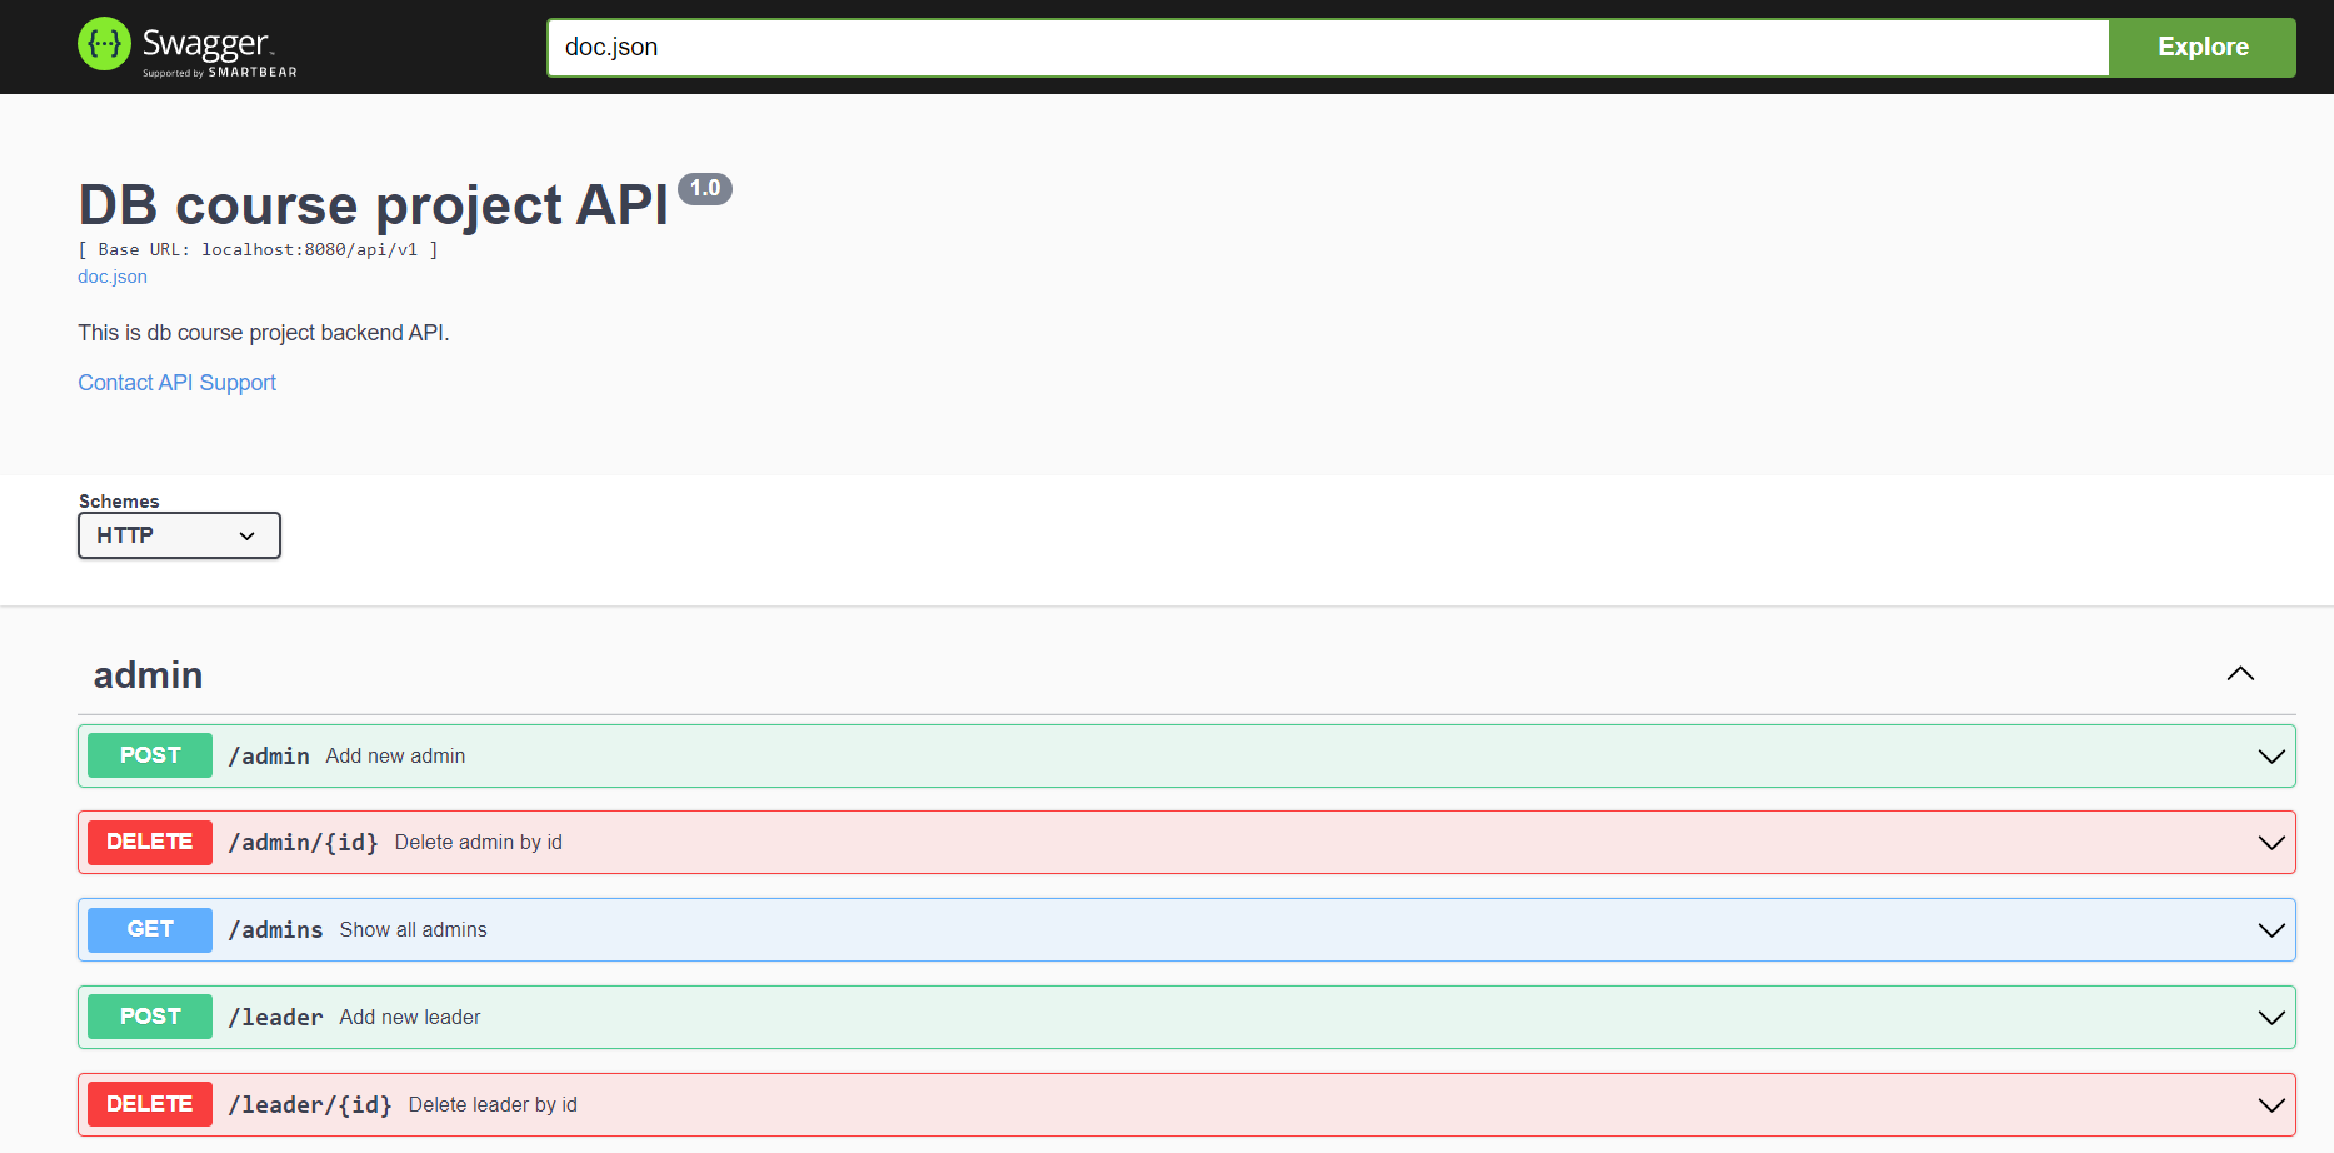
\includegraphics[width=\textwidth]{image/1.pdf}
	\caption{Главная страница}
	\label{img:page1}
\end{figure}

\begin{figure}[!h]
	\centering
	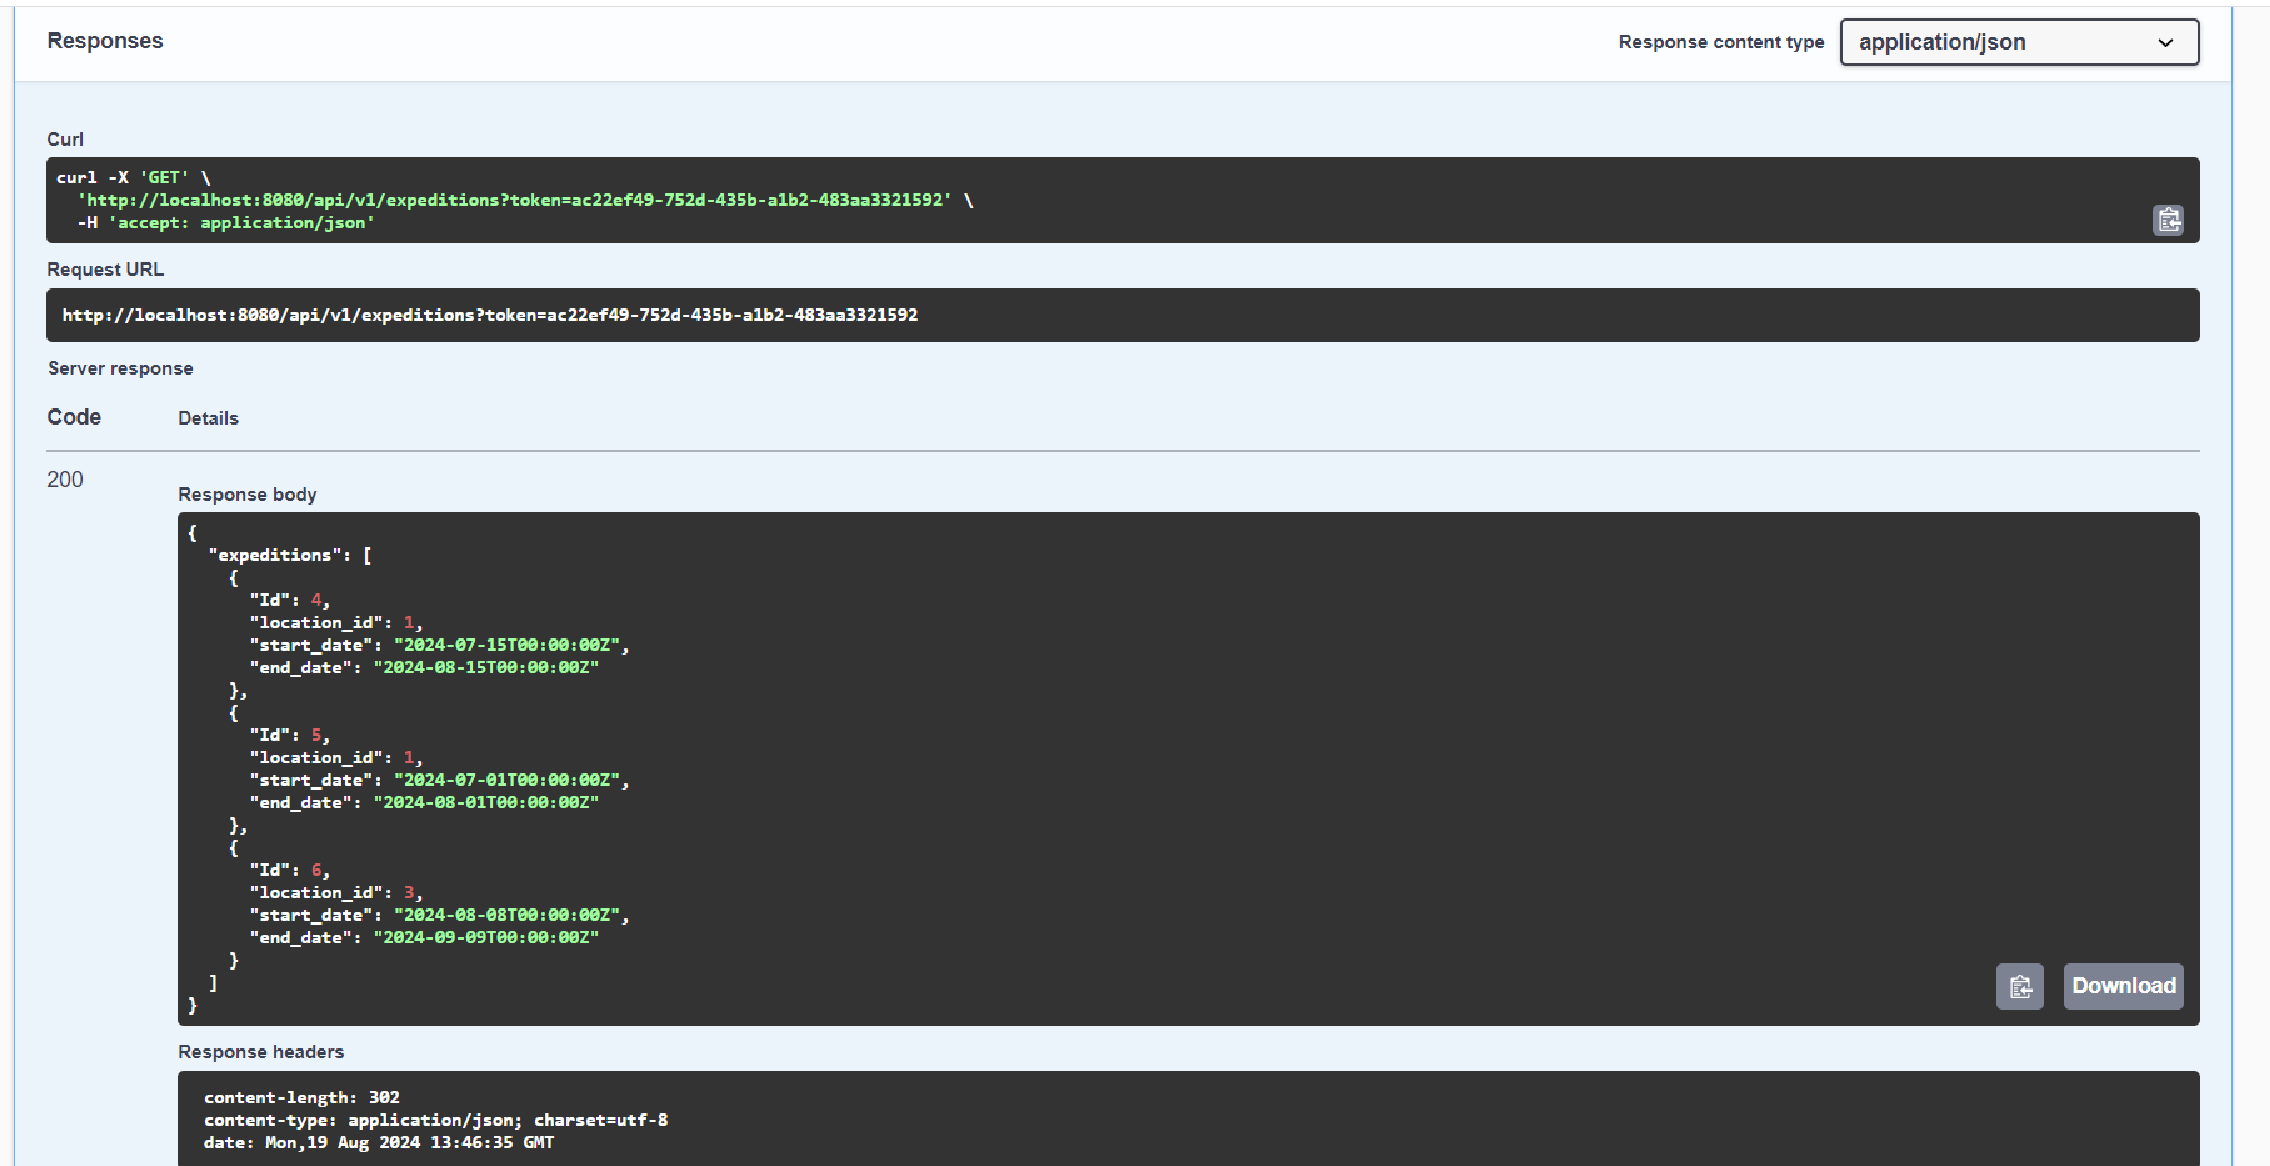
\includegraphics[width=\textwidth]{image/2.pdf}
	\caption{Пример ответа на запрос получения всех экспедиций}
	\label{img:page2}
\end{figure}


\subsection*{Вывод}
В данном разделе был проведен анализ и выбор СУБД, описаны средства и детали реализации приложения, описан интерфейс взаимодействия с приложением.

